\documentclass{acmtog} % V1.2

\let\oldquote\quote
\let\endoldquote\endquote
\renewenvironment{quote}[2][]
  {\if\relax\detokenize{#1}\relax
     \def\quoteauthor{#2}%
   \else
     \def\quoteauthor{#2~---~#1}%
   \fi
   \oldquote}
  {\par\nobreak\smallskip\hfill(\quoteauthor)%
   \endoldquote\addvspace{\bigskipamount}}

\acmVolume{1}
\acmNumber{1}
\acmYear{2018}
\acmMonth{March}
\acmArticleNum{1}
\makeatletter
\def\runningfoot{\def\@runningfoot{}}
\def\firstfoot{\def\@firstfoot{}}
\makeatother


\begin{document}

\markboth{Experimental Sentiment Analysis on Twitter}{A Real Time Stream and Big Data Process}

\title{Sentiment Analysis on Twitter : Effects in a Social Network} % title

\author{Mohamed Ben Hamdoune {\upshape and} Yannis Tannier
\affil{University of Paris-Descartes}
}

\category{H.2.8}{Database Applications}{Big Data and Real Stream}[Cloud Computing]
\category{I.3.7}{Learning}{Apache Spark and Hadoop}[Social Media Analytics]

\terms{Twitter, Psychological Profil}

\keywords{Data Mining, Natural Languages Processing, Sentiment Analysis, Classification, Text Mining}

\acmformat{Mohamed Ben Hamdoune, Yannis Tannier. 2018. Sentiment Analysis for Twitter : Effects in a Social Network.}

\maketitle

\begin{bottomstuff}
Jason Scott Sadofsky acknowledges a Jason Scott, is an American archivist, historian of technology, and filmmaker. Archive Team is a group dedicated to preserving digital history that was founded by Jason Scott in 2009. Data was collected from the website of The Archive Team.

\end{bottomstuff}


\begin{abstract}

Our purpose is to build a powerful platform for real-time data analysis of tweets on twitter trends. We also want to analyse all the tweets of 2017 based on a downloaded sample of data (average of 6To). All this data analysis will be accessible via a web interface that will be developed. We want to build a powerful system of sentiments analysis by making a database structure of tweets which is relevant about impacts and effects. The system should provide a faster way to execute Machine Learning methodologies behind data extracted from Twitter. Analysis news actuality by getting an analysis on actual trends with real stream data by building an efficient web interface to get results easily and build a system without false accounts and keep a control on data continuously.
\end{abstract}

\section{Introduction}
The main subject is \cite{Cuadros17} Sentiment Analysis on Twitter, \cite{Ayvazb17} a microblogging platform where people can easily share their thought on anything and their habits too. We have a lot of publications on sentiment analysis but not so much \cite{Marquez16} research about impacts and their effect on society. The maximum characters \cite{Jianqiang17} are 140 which can be a good thing for the process of analysis because it will make it faster in a way to perform on small messages but in the other hand we should pay attention on\cite{Meisheri17} accuracy of results. Event \cite{Jianqiang17} it’s an enormously continuous stream of data, Twitter is a good extra sentiment though an online community. Therefore, how to optimize all those streaming data \cite{Baltas17} and build a web interface for users who want to get data. Our project will \cite{Vyas17} use many methodologies from Machine Learning like unsupervised methods to make a classification of sentiments, and supervised method \cite{Palpanas11} to predicate psychological profile. Finally, one big step will be and efficient system about control of massive data incoming, a check on false account and spam messages that will destroy our \cite{Poddar16} results for example.
 
\begin{quote}{Jeffrey Zeldman}
“The best way to engage honestly with the marketplace via Twitter is to never use the words "engage," "honesty," or "marketplace." 
\end{quote}

In this study, we introduce readers to the problems of Data Processing and Cloud Computation, which have been rapidly developing over the last decade. The rest of this document is organized as follows. In Sect. 2, we provide a specific view of Tweet format. Development, problems, definitions and main trends of this area are described in Sect 3. We analyze in Sect 6, and discuss in Sect 7 about several problems we have been through.
Finally, we talk about others idea and features that were not implemented due to a lack of time in Sect 8.

\section{Related Work}
\label{sec:related_work}

To begin, ye can refer to this article \cite{Palpanas11} because we can relate that it is a point of start, it gives us a theoretical review on the development of Sentiment Analysis.
The interested reader can also refer to previous surveys in the area, like [cite] and [cite], that helped us on machine learning techniques. As an active research field that has emerged for a long time now, sentiment analysis is now been greatly implement but it is also with a cost (for example, IBM Watson Tone Analyzer). Sentiment analysis is a discipline that extracts people’s feelings, opinions, thoughts and behaviors from user’s text data using Natural Language Processing (NLP) methods. 
For methodologies on preprocessing, and feature generation, we based our work on \cite{Meisheri17} process. Then we can also cite \cite{Jianqiang17} for a reason, they removed numbers from theirs tweet thinking that in general, numbers are of no use when measuring sentiment and are removed from tweets to refine the tweet content but we wanted to keep them thinking the contrary.
Based on 36 million tweets collected from Twitter, Wang et al. proposed a real-time sentiment analysis system for classification of political tweets during 2012 US presidential elections. Their model achieved 59\% accuracy in predicting the sentiments of political tweets (Wang et al., 2012).
We had over 800 million tweets in English and all that data to analyze where possible just because of the MapReduce Model \cite{Baltas17} in majority.


\section{Methodology}
\label{sec:methodology}

Machine learning approach relies on the famous ML algorithms to solve the SA as a regular text classification problem that makes use of syntactic and/or linguistic features. Text Classification Problem Definition: We have a set of training records D  where each record is Sentiment analysis algorithms and applications: A survey labeled to a class. The classification model is related to the features in the underlying record to one of the class labels. Then for a given instance of unknown class, the model is used to predict a class label for it. The hard classification problem is when only one label is assigned to an instance. The soft classification problem is when a probabilistic value of labels is assigned to an instance.

\subsection{Pre-processing}
\label{subsub:preprocessing}

In this paper we introduce two new resources for pre-processing twitter data: 1) an emoticon dictionary and 2) an acronym dictionary. We prepare the emoticon dictionary by labeling 170 emoticons listed on Wikipedia 1 with their emotional state. For example, “:)” is labeled as positive whereas “:=(” is labeled as negative. We assign each emoticon a label from the following set of labels: Extremely-positive, Extremely-negative, Positive, Negative, and Neutral. We compile an acronym dictionary from an online resource. 2 The dictionary has translations for 5,184 acronyms. For example, lol is translated to laughing out loud. We pre-process all the tweets as follows: a) replace all the emoticons with a their sentiment polarity by looking up the emoticon dictionary, b) replace all URLs with a tag ||U ||, c) replace targets (e.g. “@John”) with tag ||T ||, d) replace all negations (e.g. not, no, never, n’t, cannot) by tag “NOT”, and e) replace a sequence of repeated characters by three characters, for example, convert coooooooool to coool. We do not replace the sequence by only two characters since we want to differentiate between the regular usage and emphasized usage of the word.

The tweets contain a lot of opinions about the data which are expressed in different ways by individuals .The twitters dataset used in this work is already labeled. Labeled dataset has a negative and positive polarity and thus the analysis of the data becomes easy. The raw data having polarity is highly susceptible to inconsistency and redundancy. The quality of the data affects the results and therefore in order to improve the quality, the raw data is pre-processed. It deals with the preparation that removes the repeated words and punctuations and improves the efficiency the data.

Step-1 Pre-Processing the tweets:
Pre-processing ()
Remove URL:
Remove special symbols
Convert to lower:
Removal of re-tweets.
 Converting upper case to lower case: In case we are
using case sensitive analysis, we might take two
occurrence of same words as different due to their
sentence case. It important for an effective analysis not
to provide such misgivings to the model.


Stop word removal: Stop words that don’t affect the
meaning of the tweet are removed (for example and,
or, still etc.). [3] uses WEKA machine learning
package for this purpose, which checks each word
from the text against a dictionary ([3], [5]).
Twitter feature removal: User names and URLs are
not important from the perspective of future
processing, hence their presence is futile. All
usernames and URLs are converted to generic tags [3]
or removed [5].



\subsection{Feature Generation}
\label{subsub:feature}

The data for this task consists of tweets across various domains, classified into four emotions: joy, sadness, anger and fear. The training data additionally carries a real-valued score between 0 and 1 per tweet, indicating the degree of the emotion (that the tweet is classified as) the present in the tweet.
The Language problem: It was noticed in the articles presented in this survey that the Far East languages especially the Chinese language has been used more often recently. Accordingly, many sources of data are built for these languages. The researchers are now in the phase of building resources of other Latin (European) languages. There is still a lack of resources for the Middle East languages including the Arabic language. The resources built for the Arabic language are not yet complete and not found easily as an open source. This makes it a very good trend of research now. NLP: The natural language processing tools can be used to facilitate the SA process. It gives better natural language understanding and thus can help produce more accurate results of SA. These tools were used to help in BR, ED and also SA task in the last two years. This opens a new trend of research of using the NLP as a preprocessing stage before sentiment analysis. Although [1] mentioned the problems of opinion aggregation and contradiction analysis, they were not found in the recent articles presented by this survey. This means that they do not attract researchers recently; despite the fact that they are still opening fields of research. It is noticed that working on domain-specific corpus gives better results than working on the domain-independent corpus. There is still lack of research in the field of domain-specific SA which is sometimes called context-based SA. This is because building the domain-specific corpus is more complicated than using the domain-independent one. It is noticed that the ED and BR task work usually on domain-independent sources, while TL always uses domain-dependent sources.


\section{Cloud Computing}
\label{sec:cloud_computing}

Cloud computing was used for the project, the trend today is machine learning, which is a form of artificial intelligence that uses algorithms to learn from data. These systems build models from incoming transactional data, then find patterns in that data to make predictions. These predictions can be a simple as providing a recommendation to a shopper on an e-commerce website or as complex as determining if a brand of automobile should be retired. As with their learning-system forebears, the overhead of machine-learning systems is typically huge. But today we have the option to place these systems in the cloud. Amazon Web Services, for example, supports machine learning using AWS's algorithms to read native AWS data (such as RDS, Redshift, and S3). Google has supported predictive analysts for some time with its Google Prediction API, and Microsoft provides an Azure machine-learning service. The ability to predict the future for both tactical and strategic purposes has eluded us because of prohibitive resource requirements. But today, thanks to the cloud for machine learning as a service, you can apply this technology far and wide on all that data enterprises have been collecting.


\subsection{Spark Framework}
\label{subsub:spark}

Here 

\subsection{Conception of the Database for the Web Interface}
\label{subsub:conception}

The World Wide Web (Web, for short), is a distributed information system based on hypertext. Web interfaces to databases have become very important. After outlining several reasons for interfacing databases with the Web, we provide an overview of Web Technology. We then applies techniques \cite{Baltas17} for building Web interfaces to databases.


\section{Implementation}
\label{sec:implementation}

We have used the following technologies for many reasons. Hadoop assumes that conventional approaches (consisting of developing ever more powerful centralized systems) have technical and financial limitations. The development of distributed systems consisting of machines or nodes, relatively affordable (commodity hardware) and scaling out is an alternative from a technical and financial point of view A distributed system comprising tens, hundreds or thousands of nodes will regularly be confronted with hardware and / or software failures. Google has developed the Google File System (GFS), ancestor of the Hadoop Disrelated File System (HDFS) and The MapReduce Approach. MapReduce is a programming model designed specifically to read, milk and write very large volumes of data. A Hadoop program usually implements both map tasks and reduce tasks.
Hadoop is particularly effective for dealing with problems that have one or more of the following characteristics: Volume of data to store or process very important. Need to perform processing on all data (batch rather than transactional, therefore). Heterogeneous data in terms of origin, structure, and format (JSON) Execute the tasks of a Hadoop job in parallel, without a pre-established order. A Hadoop cluster is made up of tens, hundreds, or thousands of nodes. It is the addition of the storage and processing capacities of each of these nodes which makes it possible to offer a storage space and a computing power yet to handle data volumes of several To or Po. To improve the performance of a read / write cluster, Hadoop’s file management system, HDFS, writes and reads files in blocks of 64 MB or 128 MB. Working on such large blocks maximizes data transfer rates by limiting search time on hard drives (seek time). // Input file graph and block MapReduce is a programming model designed specifically to read, process and write very large volumes of data. A Hadoop program usually implements both map tasks and reduce tasks. A Hadoop program is usually divided into three parts: The driver, which runs on a client machine, is responsible for configuring the job and submitting it for execution. The map is responsible for reading and processing data stored on disk. The reducer is responsible for consolidating the results from the map and write them on disk.

\section{Results}
\label{sub:results}


\begin{figure}[h!]
{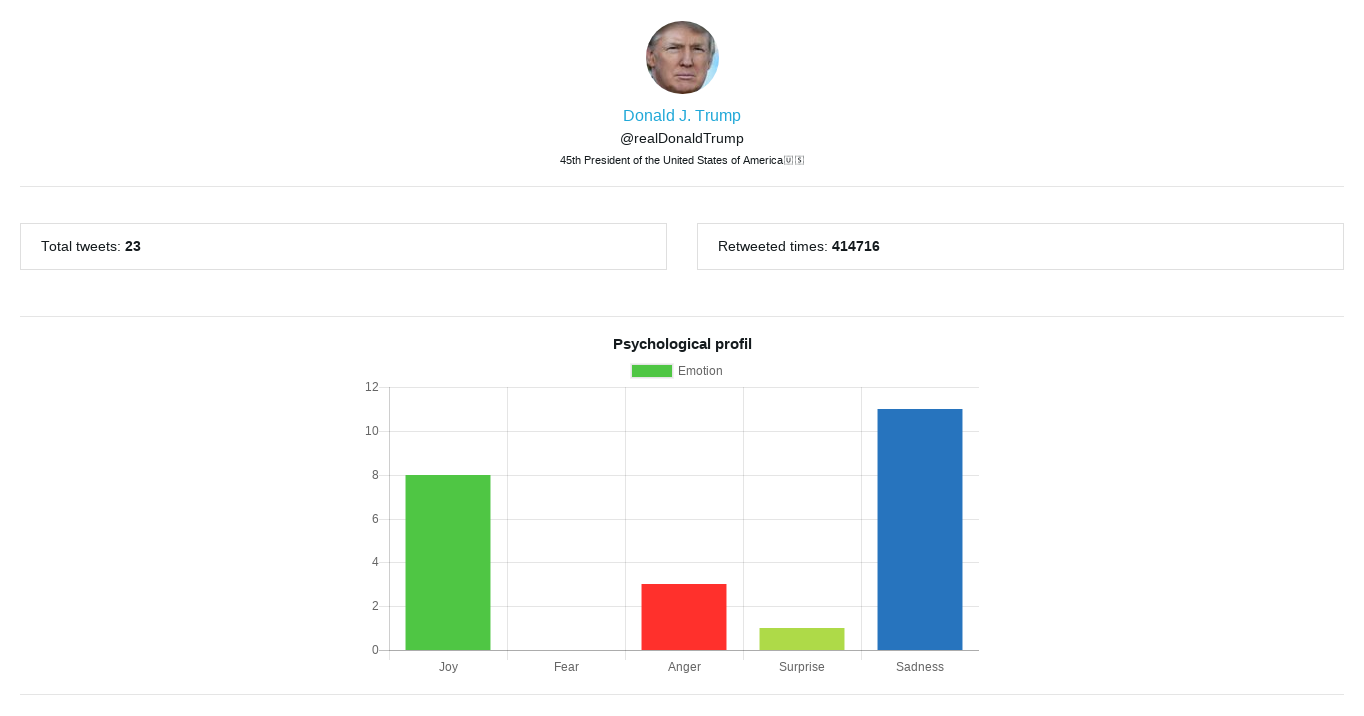
\includegraphics[width=\linewidth]{Trump-results-analysis_exemple.png}}
\caption{Results predicted by our models with Donald John Trump (born June 14, 1946), the 45th and current President of the United States.}
  \label{fig:trump_results}
\end{figure}

POMS (Profile of Mood States) is a psychological rating scale used for calculating the mood state score, the result depends on the values of 65 adjectives. For our project we reorganized the adjectives in two ways, first in 3 categories: Positive, Negative and Neutral, second way in 5 categories: Joy, Surprised, Fear, Angry, Sadness. More about the way to calculate POMS adjectives.


\begin{figure}[h!]
{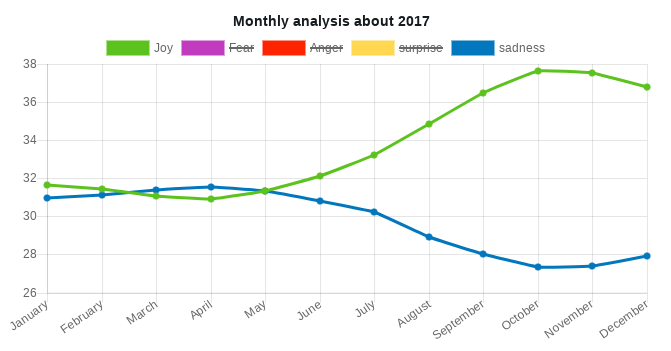
\includegraphics[width=\linewidth]{monthly_analysis_joy_sadness-exemple.png}}
\caption{Results by month for joy and sadness emotions during the 2017.}
  \label{fig:trump_results}
\end{figure}



\begin{figure}[h!]
{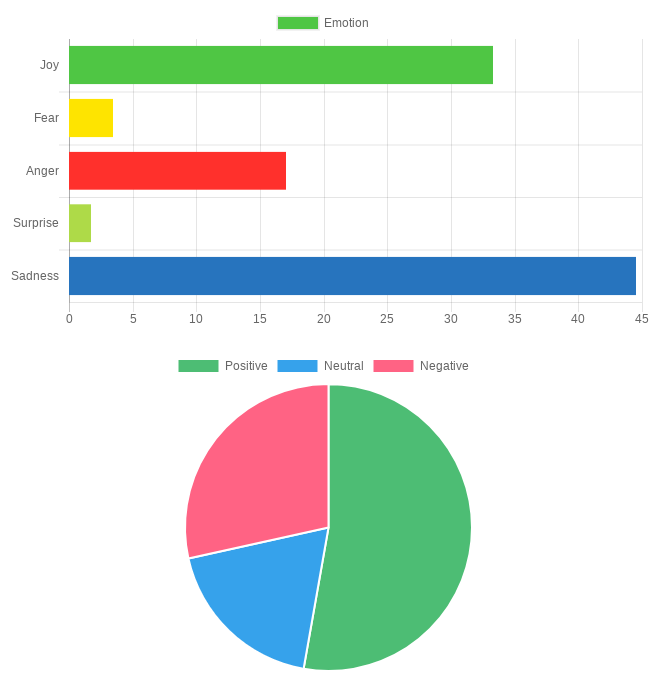
\includegraphics[width=\linewidth]{retweeted_emotion_sentiment_trump-exemple.png}}
\caption{Results for the emotions ratio on the 414 716 retweeted Donald Trump tweets computed.}
  \label{fig:trump_results}
\end{figure}


\section{Disucussion}
\label{sec:discussion}

We now turn our attention to the following interesting question: whether the subjective data that exist on the web carry useful information. Information can be thought of as data that reduce our uncertainty about some subject. According to this view, the diversity and pluralism of information on different topics can have a rather negative role. It is well understood, that true knowledge is being described by facts, rather than subjective opinions. However, this diversity in opinions, when analyzed, may deliver new information and contribute to the overall knowledge of a subject matter. This is especially true when the object of our study is the attitude of people. In this case, opinion native data can be useful to uncover the distribution of sentiments across time, or different groups of people.
The term data mining refers loosely to process of semiautomaticcally analyzing large databases to find useful patterns. Like knowledge discovery in artificial intelligence (also called machine learning) or statistical analysis, we use data mining to discover rules and patterns from data. However, data mining differs from machine learning and statistics in that it deals with large volumes of data, stored primarily on disk. That is, data mining deals with “knowledge discovery in databases”. Some types of knowledge discovered from a database can be represented by a set of rules. The following is an example of a rule, stated informally: “Donald Trump with his totals of retweets incomes are greater than the average with the most sadly effects on users”. Of course, such riles are not universally true, and have degrees of “support” and “confidence”, as we shall see. Other types of knowledge are represented by equations relating different variables to each other, or by other mechanisms for predicting outcomes when the values of some variables are known. There are a variety of possible types of patterns that may be useful, and different techniques are used to find different types of patterns. Usually there is a manual component to data mining, consisting of preprocessing data to a form acceptable to the algorithms and postprocessing of discovered patterns. For this reason, data mining is really a semiautomatic process in real life. The mode widely used applications are those that requires some sort of prediction. In our case, we want to predict emotions and sentiments, then a psychological profile. Prediction is one of the most important types of data mining. We outline what is classification, study techniques for building one type of classifiers, called decision-tree classifiers, and then study other predication techniques. Abstractly, the classification problem is this: Given that user belong to the archive, and given his tweet. We use a given instances (called training instances) of items along with the classes to which they belong, the problem is to predict the class (in our study it is a sentiment or an emotion) to which a new item belongs.
This is an example with a sample of 383 623 424 tweets in English.

\begin{table}[h!]

\tbl{Cross Tab for sentiments and emotions}{%
\begin{tabular}[width=\linewidth]{rcrcrcrcrcrc@{0.5in}}
S\textbackslash E &{Joy} &{Fear} &{Anger} &{Surprise} &{Sadness} \\
$Positive$ & 63 559 579 & 9 296 846 & 27 861 247 & 7 768 707 & 42 382 993  \\
$Neutral$ & 55 127 659 & 15 777 833 & 42 460 015 & 8 879 626 & 48 232 835 \\
$Negative$ & 9 054 496 & 3 395 622 & 23 281 712 & 1 948 578 & 24 595 676 \\
\end{tabular}}
\label{tab:cross_tab}
\end{table}


\section{Conclusion and Future Work}
\label{sec:conclusion}

In this report we have presented a\cite{Lin18} sentiment analysis tool on a\cite{Medhat14} Web interface, in one hand we used data from an archive end in the other we used real time stream analysis. Due\cite{Rebecca11} to the absence of labelled data we couldn’t discuss the accuracies of the two enhancements. In the future\cite{Gautam14}, we plan to use the\cite{Badhani17} as feedback mechanism to classify new tweets.

% Start of "Sample References" section

\section{References}

\begin{acks}
We are grateful to the following people for resources, discussions and suggestions: Jason Scott (Archivist) and Diana Yuan (Co-Founder & Vice President, Talent & Operations from Indico).
\end{acks}


% Bibliography

\bibliographystyle{ACM-Reference-Format-Journals}
\bibliography{publication-bibfile}

\end{document}